% =============================================================
%  國立高雄科技大學 資訊工程學系 — 專題報告
%  編譯方式：Overleaf 右上角 Menu → Compiler 選 "XeLaTeX"
%            （ctex 套件需要 XeLaTeX，不可用 pdfLaTeX）
%  中文字型：主字型使用標楷體；Overleaf / Arch Linux 編譯器請選 XeLaTeX
% =============================================================
\documentclass[12pt, a4paper, fontset=none]{ctexart}

% ---------- 中文字型（Overleaf / XeLaTeX）----------
% 主字型優先指定為標楷體字型檔（Windows 常見檔名：DFKai-SB.ttf）。
% Arch Linux 若未安裝合法標楷體字型檔，則使用 Noto Serif CJK TC 作為可完整覆蓋繁中字元的編譯 fallback；
% 若要強制使用真正標楷體，請將 DFKai-SB.ttf 放入 ~/.local/share/fonts/ 後執行 fc-cache -fv。
\IfFontExistsTF{DFKai-SB.ttf}{
  \setCJKmainfont{DFKai-SB.ttf}[AutoFakeBold=true,AutoFakeSlant=true]
}{
  \setCJKmainfont{Noto Serif CJK TC}[AutoFakeBold=true,AutoFakeSlant=true]
}
\setCJKsansfont{Noto Sans CJK TC}[AutoFakeBold=true,AutoFakeSlant=true]
\setCJKmonofont{Noto Sans Mono CJK TC}

% ---------- 版面 ----------
\usepackage[top=2.5cm, bottom=2.5cm, left=3cm, right=3cm]{geometry}
\usepackage{setspace}
\onehalfspacing                       % 1.5 倍行距

% ---------- 數學 ----------
\usepackage{amsmath, amssymb, amsfonts}
\usepackage{bm}

% ---------- 圖表 ----------
\usepackage{graphicx}
\usepackage{float}
\usepackage{booktabs}
\usepackage{multirow}
\usepackage{array}
\usepackage{tabularx}
\usepackage{caption}
\usepackage{subcaption}
\captionsetup{font=small, labelfont=bf}

% ---------- 程式碼 ----------
\usepackage{listings}
\usepackage{xcolor}
\definecolor{codegray}{rgb}{0.95,0.95,0.95}
\definecolor{codekey}{rgb}{0.0,0.3,0.6}
\definecolor{codecomment}{rgb}{0.3,0.5,0.3}
\lstset{
  basicstyle=\ttfamily\small,
  backgroundcolor=\color{codegray},
  keywordstyle=\color{codekey}\bfseries,
  commentstyle=\color{codecomment}\itshape,
  numbers=left, numberstyle=\tiny\color{gray},
  breaklines=true, frame=single, framesep=4pt,
  showstringspaces=false, captionpos=b,
}

% ---------- 超連結（放最後載入）----------
\usepackage[colorlinks=true, linkcolor=black, citecolor=blue, urlcolor=blue]{hyperref}

% ---------- 自訂指令 ----------
\newcommand{\code}[1]{\texttt{#1}}

% ---------- 繁體中文標籤覆寫（ctex 預設為簡體：插图／图／目录／参考文献）----------
\AtBeginDocument{%
  \renewcommand{\contentsname}{目錄}%
  \renewcommand{\listfigurename}{圖目錄}%
  \renewcommand{\listtablename}{表目錄}%
  \renewcommand{\figurename}{圖}%
  \renewcommand{\tablename}{表}%
  \renewcommand{\refname}{參考文獻}%
  \renewcommand{\abstractname}{摘要}%
  \renewcommand{\appendixname}{附錄}%
}

% =============================================================
%  封面
% =============================================================
\begin{document}

\begin{titlepage}
\centering
\vspace*{2.4cm}
{\Large \textbf{國立高雄科技大學}\par}
\vspace{0.45cm}
{\large \textbf{資訊工程學系}\par}

\vspace{2.4cm}
{\normalsize 專題名稱\par}
\vspace{0.75cm}
{\LARGE \textbf{基於 eBPF Fast Path 之}\par}
\vspace{0.45cm}
{\LARGE \textbf{低延遲 DDoS 偵測與緩解系統}\par}

\vspace{2.6cm}
{\normalsize \textbf{專題隊員}\par}
\vspace{0.45cm}

{\small
\setlength{\tabcolsep}{6pt}
\renewcommand{\arraystretch}{1.35}
\begin{tabular}{|c|c|l|l|}
\hline
\textbf{姓名} & \textbf{學號} & \textbf{E-mail} & \textbf{負責項目說明} \\
\hline
黃欣怡 & C112151130 & C112151130@nkust.edu.tw & 成果展現、報告撰寫 \\
\hline
方柏翰 & C112151143 & C112151143@nkust.edu.tw & 模型製作、報告撰寫 \\
\hline
楊玉蠳 & C112151161 & C112151161@nkust.edu.tw & 模型驗證、報告撰寫 \\
\hline
\end{tabular}
}

\vfill
{\normalsize 指導教授：王志強教授\par}
\vspace{1.1cm}
{\normalsize 中華民國 115 年 08 月 19 日\par}
\end{titlepage}

\newpage
\section*{摘要}
分散式阻斷服務攻擊（Distributed Denial of Service, DDoS）會以大量封包消耗服務資源，防禦系統因此必須在極低延遲下完成早期判斷。然而，完整機器學習模型難以直接部署於 Linux 核心資料路徑（kernel datapath）：eBPF 程式受到驗證器（verifier）、無浮點運算、有限堆疊與有界迴圈等限制，無法在封包快速路徑（fast path）中執行完整樹狀模型。因此，本專題的核心訴求並非提出最高準確率的離線 DDoS 分類器，而是建立一套可部署於 Linux eBPF fast path 的 DDoS 偵測與初步處置管線。本系統以 Contract5 feature contract 限制部署特徵必須可由資料路徑重建，並以 quantile-bucket distillation 將 continuous teacher 壓縮為 5-bit bucket student 與 32-entry 評分表（score table），使核心端推論可化為整數比較與常數時間查表。

系統採回饋式分層架構：XDP 負責早期封包解析、黑名單檢查、SYN flood 相關處理，並在目前實作中執行 Contract5 特徵重建、分位桶索引與分數查表；TC 保留為資料路徑延伸與 classifier 掛載點；Rust 使用者空間（userspace）負責載入模型參數、寫入 BPF map、記錄事件，並支援防污染的雙草圖閘控邊界更新。實驗以 CIC-IDS-2019 為評估範圍，並固定於誤報率（FPR）低於 1\% 的操作點評估部署模型，而非以最佳化於測試集的離線門檻宣稱效果。結果顯示，deployed student 對多種 UDP 反射／放大型 DDoS 具良好偵測能力，但 Syn、UDP-lag 與 WebDDoS 仍屬盲區；跨資料集結果則僅作為分佈轉移與限制分析，而非主要成功標準。整體而言，本專題的貢獻在於建立 Python 離線模型、Rust 控制面與 eBPF XDP／TC 資料路徑之間可驗證、可部署且操作點明確的低延遲偵測與初步處置管線。

\vspace{1em}
\noindent\textbf{關鍵字：} 分散式阻斷服務攻擊、eBPF、異常偵測、Isolation Forest、kernel datapath、quantile-bucket distillation、lookup inference

\newpage
\tableofcontents
\listoffigures
\listoftables
\newpage

% =============================================================
\section{導論}
\label{sec:intro}

\subsection{計畫背景}
隨著網路服務高度依賴即時可用性，分散式阻斷服務攻擊（Distributed Denial of Service, DDoS）仍是影響線上服務穩定性的主要威脅之一。以 Cloudflare 的網路觀測資料為例，其在 2025 年第一季阻擋 2,050 萬次 DDoS 攻擊，較前一年同期增加 358\%，其中網路層 DDoS 達 1,680 萬次；同一份報告亦指出，約 89\% 的第三、四層 DDoS 攻擊在 10 分鐘內結束~\cite{cloudflare2025q1ddos}。這些資料顯示，DDoS 防禦不只需要辨識攻擊流量，也需要在短時間內自動完成放行、監控、限流或丟棄等決策。若偵測邏輯只能在使用者空間（userspace）以高延遲方式執行，即使模型具有良好離線準確率，也可能無法在攻擊高峰期間即時保護服務。

機器學習異常偵測方法能從正常流量分布中學習異常模式，對於規則難以完整列舉的流量型攻擊具有應用潛力。然而，本研究關注的核心問題並非單純追求最高的機器學習準確率，而是在於：如何將可部署的異常偵測邏輯轉換為可直接於 Linux 核心資料路徑（kernel datapath）執行的輕量化防禦機制。eBPF 程式雖能在 XDP／TC 等掛載點（hook）提供低延遲封包處理能力，但其驗證器（verifier）會檢查控制流程、暫存器／堆疊狀態與記憶體存取安全，並拒絕不符合安全條件的程式~\cite{linuxBpfVerifier}。因此，系統必須在追求高吞吐效能的同時，將模型推論轉換為驗證器友善的整數運算與 BPF map 查表。

需先界定的是，本專題目前以 CIC-IDS-2019 作為主要實驗與部署評估範圍。BigFlow、IDS2018 HOIC 與 LOIC-HTTP 等結果則作為分佈轉移（distribution shift）與模型限制之輔助分析，而非主要成功標準。系統現況唯一的執行期（runtime）推論層為 eBPF 快速路徑；完整孤立森林（Isolation Forest）僅作為離線 teacher / reference model，尚未接入執行期。

\subsection{研究動機}
基於上述背景，本專題的研究動機可歸納為以下三項：

\begin{enumerate}
  \item \textbf{使用者空間機器學習推論與核心快速路徑需求之落差。} 傳統網路入侵偵測系統（NIDS）或機器學習式 DDoS 偵測多在使用者空間完成特徵組裝與模型推論，雖可使用完整資料結構、浮點運算與複雜模型，但在高封包率攻擊下，跨越核心／使用者空間邊界與完整模型推論成本可能成為即時防禦瓶頸。相較之下，eBPF 可於 XDP／TC 掛載點進行早期封包處理，但其驗證器對控制流程、記憶體存取與堆疊使用有嚴格要求。因此，本專題希望將離線異常偵測邏輯壓縮為 eBPF 可接受的整數比較與常數時間查表。

  \item \textbf{可由資料路徑重建的輕量統計特徵需求。} 若部署模型依賴高維流特徵或需要完整封包歷史，則難以在核心快速路徑中重現。本專題因此聚焦於不檢查酬載（payload）、可由 L3／L4 封包與連線狀態（session state）累積的統計特徵，例如協定、平均封包長度、前向最大封包比例、方向對稱性與封包長度變異係數。這些特徵必須能以整數運算或交叉乘法表示，才能符合 eBPF 無浮點與低延遲的限制。

  \item \textbf{自適應邊界更新中的攻擊污染風險。} 在長時間部署情境中，流量分布可能因正常業務型態改變而產生漂移，因此防禦邊界需要具備校準能力。然而，若串流更新（streaming update）不區分良性漂移（benign drift）與攻擊污染（attack contamination），攻擊流量可能被納入參考分布，使系統逐漸將攻擊校準為正常。本專題因此將自適應邊界校準放在使用者空間回饋層，透過雙草圖閘控更新（dual-sketch gated update）與 AttackFreeze 狀態隔離攻擊污染，而非在封包快速路徑中進行完整模型重訓。
\end{enumerate}

\subsection{研究問題}
基於上述動機，本研究針對 eBPF-based DDoS fast-path 部署中的四項實務問題進行評估與求解：

\begin{enumerate}
  \item \textbf{離線異常偵測邏輯與 eBPF 相容性。} 如何將離線孤立森林所代表的異常偵測邏輯與 Contract5 特徵空間，轉換為僅需整數比較與查表即可完成推論的 5-bit 全二值化分位桶策略，而不在核心快速路徑中執行完整樹狀模型。

  \item \textbf{特徵整數化與比例比較。} 在 eBPF 不適合浮點運算與高成本除法的前提下，如何運用可由連線狀態累積的統計量，並以整數比較與交叉乘法取代比例特徵中的除法與浮點比較。

  \item \textbf{資料路徑分工與效能隔離。} 如何協同 XDP、TC 與使用者空間：目前實作將封包解析、黑名單、SYN-cookie、狀態更新與分位桶查表集中於 XDP fast path，TC 保留為 classifier 擴充掛載點；此設計需避免讓完整樹狀模型或高成本邏輯進入 per-packet fast path。

  \item \textbf{適應性邊界校準與攻擊污染隔離。} 如何於使用者空間透過雙草圖閘控更新支援分位桶邊界校準，同時區分良性漂移與攻擊污染，避免串流更新將攻擊流量校準為正常；並透過具版本號的雙緩衝 BPF map 確保熱更新過程中資料路徑參數一致性。
\end{enumerate}

\subsection{本專題之工程貢獻}
本專題的核心訴求不是單純訓練一個 DDoS 偵測模型，而是研究如何將離線異常偵測模型安全、低延遲且可驗證地部署到 Linux eBPF fast path。基於此定位，本專題之工程貢獻與實驗觀察如下：

\begin{enumerate}
  \item \textbf{提出 Contract5 feature contract。} 本專題將離線流量特徵收斂為五個可由 L3／L4 封包欄位與核心連線狀態重建的 Contract5 特徵，並定義特徵順序、位元順序、長度單位、評分表與分位桶邊界等格式，使 Python 離線流程、Rust 使用者空間載入器與 eBPF 評分器能依相同規格運作。此貢獻重點不在於提出全新特徵，而在於將機器學習特徵空間轉換為資料路徑可重建、可整數化且可驗證的部署 contract。

  \item \textbf{以 quantile-bucket distillation 形成 fast-path lookup inference。} 完整孤立森林不適合直接部署於 eBPF，因此本專題以 $N=2$ 分位桶將五個 Contract5 特徵轉換為 5-bit 索引，並以 32-entry bucket student 評分表取代樹狀巡訪，使 kernel fast path 僅需整數比較與 BPF map lookup。在 CIC-DDoS2019 的 FPR $\leq 1\%$ 操作點上，deployed student 達 F1 = 0.901、Recall = 0.821。分位桶數量掃描實驗亦顯示，$N=4$ 在低 FPR 操作點崩潰，而 $N=8$ 需 32768-entry 表；因此 $N=2$ 是目前操作點穩健性與 eBPF 可行性之間的合理折衷。

  \item \textbf{設計 XDP／TC／userspace 分層管線。} 本專題整合 Python 離線訓練與模型匯出、Rust 使用者空間的模型載入器／記錄器／邊界更新器（BoundaryUpdater），以及 eBPF XDP／TC 資料路徑。目前實作中，XDP 負責封包解析、黑名單檢查、SYN flood 相關處理、連線狀態更新與 Contract5 評分表查表；TC 保留為 classifier 擴充掛載點；使用者空間則負責模型參數下發、事件記錄與邊界校準，使封包快速路徑、模型載入與策略更新各自位於合適層級。

  \item \textbf{在低 FPR 操作點下評估部署模型有效範圍。} 本專題以 CIC-IDS-2019 為主要範圍，在 FPR $\leq 1\%$ 操作點下比較 Contract5 continuous teacher、Abs20 baseline、deployed binarized student 與 supervised reference，並逐攻擊類型揭露有效範圍與盲區。此貢獻避免只以離線 AUC 或最佳 threshold 描述效果，而是將模型評估對齊 DDoS 防禦中正常流量不可大量誤擋的實務要求。

  \item \textbf{設計防攻擊污染的邊界更新機制並明確界定限制。} 本專題將雙草圖閘控更新整合至使用者空間回饋層，以區分正常流量漂移與攻擊污染。實驗顯示，樸素串流更新（naive streaming update）在攻擊比例 $\rho \geq 30\%$ 時漏報率（FNR）上升至 1.000，而閘控更新可透過 AttackFreeze 將 FNR 維持於基準值 0.182。同時，本專題明列 Syn、UDP-lag、WebDDoS 與跨資料集 HOIC／BigFlow 等範圍外或盲區案例，使成果定位於可驗證的 kernel fast-path 實作，而非未受限制的泛化能力宣稱。
\end{enumerate}

% =============================================================
\section{既有技術與相關研究}
\label{sec:related}

本專題位於兩類既有技術的交界：一方面，傳統機器學習式網路入侵偵測系統（ML-based NIDS）研究涵蓋多種網路攻擊偵測任務，DDoS 偵測是其中之一，此類研究多聚焦於資料集、特徵選取與分類或異常偵測準確率；另一方面，eBPF／XDP 相關工作則強調在核心資料路徑中進行低延遲封包處理。前者通常未處理完整模型於 eBPF 驗證器限制下的部署問題，後者則不一定提供可由離線機器學習流程對齊的模型部署規格。本章先回顧兩類研究，再說明本專題與既有技術之取捨。

\subsection{機器學習式入侵偵測與 DDoS 偵測}
大規模 NIDS 資料集與特徵工程研究提供了模型訓練與評估基礎。例如 BigFlow-NIDS 建構了包含 66{,}935{,}021 條流量紀錄的大型樣本庫~\cite{uddin2026bigflow}，而特徵選取研究亦整理了 NIDS 中常見的過濾式（filter）、包裹式（wrapper）與嵌入式（embedded）方法~\cite{verma2022feature}。在 DDoS 偵測方面，既有碩士論文研究已嘗試以監督式機器學習進行分散式阻斷服務攻擊偵測~\cite{sun2019ml}，以自編碼器重構誤差結合孤立森林偵測未知型 DDoS~\cite{zhao2024autoencoder}，並以深度神經網路搭配特徵優化提升偵測效果~\cite{wu2024dnn}。這些研究印證了異常偵測與孤立森林在 DDoS 場景的可行性，但其推論皆於使用者空間以完整模型執行，未處理核心資料路徑的部署限制。本專題承接此類工作對流層級（flow-level）特徵與孤立森林的重視，但將評估範圍收斂於 CIC-IDS-2019，並將重心移至核心快速路徑的可部署性。

\subsection{eBPF／XDP 資料路徑與其限制}
eBPF 可於 XDP／TC 等掛載點提供低延遲封包處理能力，已被應用於輕量級監控與執行期防禦。例如，已有研究將 eBPF 應用於物聯網環境的輕量監控機制~\cite{lai2022ebpf}，亦有工作以 eBPF 在 Linux 容器中進行語意層級 DDoS 攻擊的執行期偵測~\cite{remya2025ebpf}。然而，eBPF 的驗證器會檢查控制流程、暫存器／堆疊狀態與記憶體存取安全，並拒絕不符合安全條件的程式~\cite{linuxBpfVerifier}；相關研究也指出 eBPF 網路程式在 JIT、SIMD、記憶體操作與輔助函式（helper）使用上存在不同於原生核心模組的效能限制~\cite{shahinfar2025demystifying}。因此，完整樹狀模型或高維浮點特徵不適合直接置入核心快速路徑，必須轉換為小型、整數化、可查表的部署形式。

\subsection{特徵標準化、特徵縮減與跨環境限制}
既有研究指出，網路安全資料集之間存在特徵定義、尺度與資料收集環境不一致等問題，因此特徵標準化與跨資料集比較需謹慎處理~\cite{moyano2023feature}。另一方面，近期 IoT NIDS 研究亦顯示，feature reduction 是降低模型計算成本與延遲的重要方法。Li 等人以 Network TON-IoT 資料集比較 feature selection 與 feature extraction，並同時評估 accuracy、F1-score、training time 與 inference time；其研究指出，feature selection 與 feature extraction 在偵測表現與執行成本上具有不同取捨，且 feature extraction 雖能在部分低特徵數設定下取得較佳偵測表現，但也會將原始欄位投影至新的低維空間，使特徵語意較不直覺~\cite{li2024featureReduction}。

本專題實驗亦觀察到，若部署模型高度依賴絕對流量規模，跨資料來源評估時容易受到環境差異影響。因此，本系統將主成果限定於 CIC-IDS-2019 範圍內評估，並將跨資料集結果視為限制分析，而非泛化能力宣稱。對 eBPF fast path 而言，特徵縮減不只涉及離線模型準確率，也涉及特徵是否能由 L3/L4 封包欄位與 kernel session state 重建、是否能整數化、以及是否能以 BPF map 查表形式部署。因此，本專題採用 deployment-constrained feature selection / feature contract 的思路，保留可由 datapath 重建且可驗證的 Contract5，而非採用 PCA 類 feature extraction。

\subsection{比較分析}
\paragraph{核心對比 A：準確率導向模型與部署導向模型。}
傳統機器學習式 NIDS 常以離線分類準確率、AUC 或特徵重要性作為主要評估目標；然而，在 eBPF DDoS 快速路徑場景中，模型是否能被驗證器接受、是否能以有界整數運算執行、以及是否能在低 FPR 操作點下穩定決策，同樣是設計核心。因此，本專題不以高維模型的最佳離線 AUC 作為唯一標準，而是將可部署性納入模型設計本身。

\paragraph{核心對比 B：部署規格與特徵表示。}
相較於僅在離線流程中選出高分特徵，本系統要求每一個特徵皆可由 eBPF 連線狀態重建，並可轉換為整數比較或分位桶邊界。Contract5 包含 \code{protocol}、\code{pkt\_len\_mean}、\code{fwd\_max\_q}、\code{sym\_ratio} 與 \code{pkt\_cv\_sq} 五個特徵，如表~\ref{tab:features} 所示。此處的「部署規格」重點是 Python--Rust--eBPF 對齊與核心可執行性，不應解讀為已完成跨資料集泛化。

\begin{table}[H]
  \centering
  \caption{Contract5 部署規格特徵與 eBPF 表示方式}
  \label{tab:features}
  \small
  \renewcommand{\arraystretch}{1.2}
  \setlength{\tabcolsep}{4pt}
  \begin{tabularx}{\textwidth}{>{\raggedright\arraybackslash}p{0.25\textwidth} >{\raggedright\arraybackslash}p{0.24\textwidth} X}
    \toprule
    \textbf{特徵} & \textbf{公式 / 定義} & \textbf{eBPF 表示方式與用途} \\
    \midrule
    \code{protocol} & L4 協定 & 由封包標頭解析後二值化，用於區分 TCP／UDP 等基礎協定差異 \\
    \code{pkt\_len\_mean} & 封包長度平均 & 由連線累積封包長度與封包數，以整數方式比較分位桶邊界 \\
    \code{fwd\_max\_q} & Fwd max / Fwd mean & 以前向最大封包長度與平均長度形成比例，部署時以交叉乘法避免除法與浮點數 \\
    \code{sym\_ratio} & Fwd pkts / Bwd pkts & 描述前向與後向封包數不對稱性，用於捕捉單向或高度偏斜流量 \\
    \code{pkt\_cv\_sq} & $(\text{Std} / \text{Mean})^2$ & 以平方形式保留封包長度變異資訊，避免核心中開根號與浮點運算 \\
    \bottomrule
  \end{tabularx}
\end{table}

\paragraph{核心對比 C：資料路徑掛載點分工。}
既有 eBPF DDoS 防禦多強調 XDP 的早期丟棄能力；然而，所有邏輯皆放入 XDP 可能使最早期封包路徑承擔過多狀態與推論成本。本專題早期設計採 XDP／TC 分工，將早期阻斷與模型評分分置於不同掛載點；目前可執行實作則將 Contract5 評分器收斂於 XDP fast path，以便量測完整 bucket 資料路徑成本，並將 TC 保留為後續 classifier 擴充位置。此取捨使目前成果更接近「單一 XDP fast path 可部署雛形」，而非已完成所有掛載點分層最佳化。

% =============================================================
\section{理論設計}
\label{sec:theory}

\subsection{防禦目標}
本系統主要鎖定可由 L3／L4 流統計特徵表徵的高流量型（volumetric）DDoS，特別是 CIC-IDS-2019 中的 UDP 反射／放大（reflection／amplification）類型攻擊，例如 DNS、LDAP、MSSQL、NTP、NetBIOS、SNMP、SSDP、UDP 與 TFTP 等高流量攻擊。此類攻擊通常會在封包大小、方向對稱性、協定分布與流統計上形成可由 Contract5 特徵捕捉的異常模式，因此適合交由 eBPF 快速路徑進行低延遲篩選。對於 SYN flood 類型攻擊，本系統另以 XDP SYN-cookie 路徑作為補充防線，而非完全依賴分位桶評分器。

\subsection{攻擊者能力假設}
本研究假設攻擊者可產生大量封包或連線，並可能在短時間內造成流統計分布偏移。攻擊者不需要控制防禦端的使用者空間程式，只要攻擊流量進入取樣視窗，即可能污染樸素的串流邊界更新，使攻擊分布被逐步校準為新常態。因此，回饋層的安全重點在於區分正常流量漂移與攻擊污染，避免攻擊流量被誤納入參考邊界。

另一方面，本研究假設防禦端主機與控制面仍屬可信任運算基礎（Trusted Computing Base, TCB）：攻擊者無法取得 root 權限，也無法直接修改 eBPF 程式、BPF map 內容或 Rust 使用者空間設定。若主機已被入侵、控制面憑證外洩，或攻擊者可直接寫入 BPF map，則超出本專題威脅模型。

\subsection{非目標與限制邊界}
本專題目前不宣稱解決所有 DDoS 型態，限制邊界如下：

\begin{itemize}
  \item \textbf{SYN flood：} 由獨立 XDP SYN-cookie 路徑處理，不作為分位桶評分器的主要偵測指標。
  \item \textbf{UDP-lag：} 屬 Contract5 快速路徑的已知盲區，目前需要不同特徵或更細緻的流量行為建模。
  \item \textbf{WebDDoS／LOIC-HTTP 等應用層洪水：} 可能需要 HTTP 方法、URL 長度、請求樣式或應用層行為特徵，超出目前 L3／L4 資料路徑規格。
  \item \textbf{跨資料集泛化：} BigFlow、IDS2018 HOIC 等資料集目前作為分佈轉移與限制分析，不作為本專題主要成功標準。
  \item \textbf{主機入侵與控制面妥協：} 若攻擊者已取得防禦端主機權限或可修改 eBPF map，則不在本研究處理範圍內。
\end{itemize}

% =============================================================
\subsection{系統架構}
\label{sec:design}

\subsubsection{系統架構圖}
\begin{figure}[H]
  \centering
  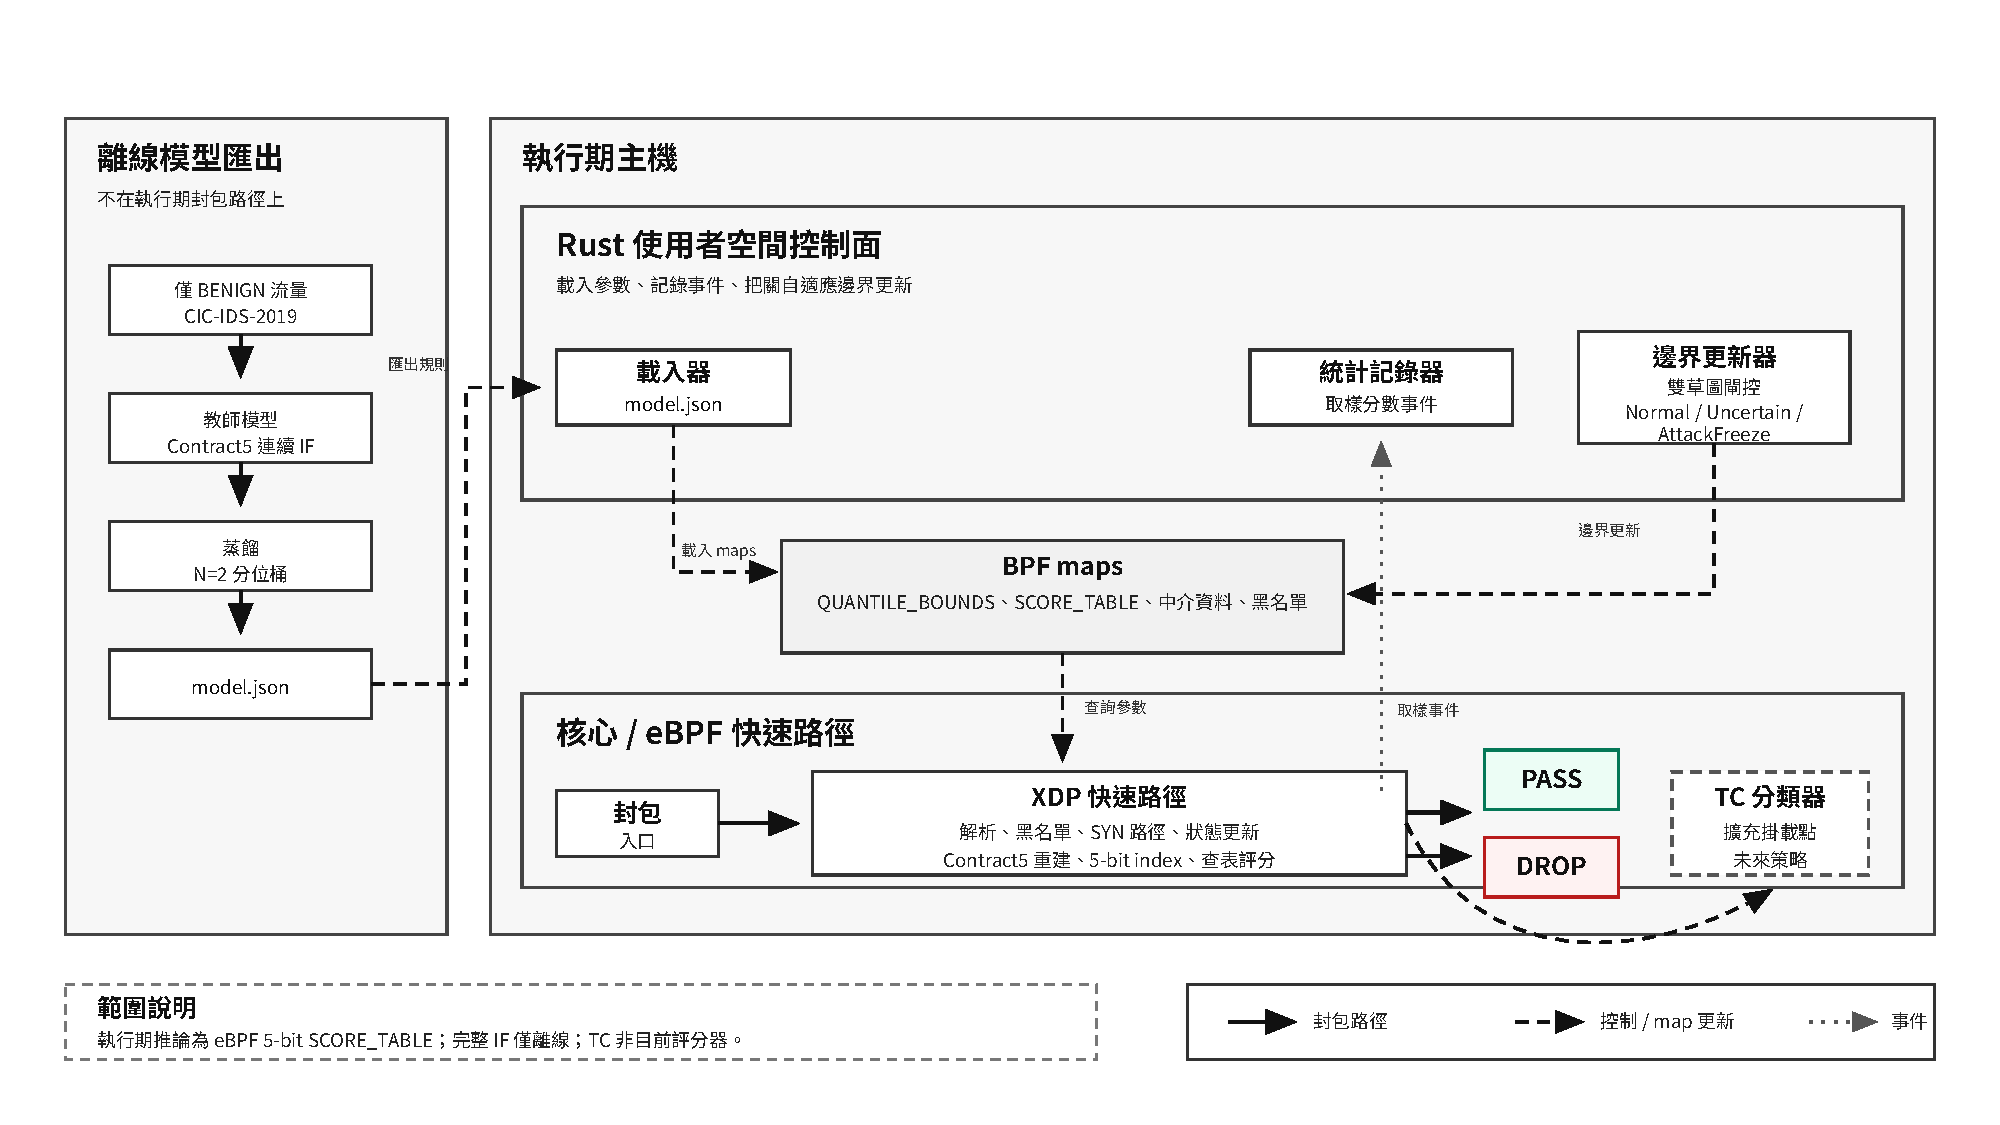
\includegraphics[width=0.95\textwidth]{figures/architecture.pdf}
  \caption{系統整體回饋式架構。XDP／TC 構成核心資料路徑；目前實作中 XDP 執行封包解析、狀態更新與 32-entry score table 查表，TC 保留為 classifier 擴充掛載點；Rust 使用者空間負責模型參數下發、日誌與邊界校準；完整孤立森林不在執行期資料路徑中執行。}
  \label{fig:arch}
\end{figure}

\subsubsection{資料流程說明}
封包進入系統後，首先由 XDP 快速路徑進行封包解析、黑名單比對、SYN-cookie 相關處理與連線狀態更新；目前實作亦在 XDP 中重建部署規格所需的五個特徵，依分位桶邊界轉換為 5-bit 索引，並查詢 32-entry 評分表取得異常分數。現況部署路徑以 \code{score >= threshold} 觸發 \code{DROP}，未達門檻則 \code{PASS}；\code{MONITOR} 與 \code{RATE\_LIMIT} 保留為後續 score-to-action policy 擴充，而非本報告主要實測結果。TC 掛載點目前保留為 classifier 擴充位置。回饋層則位於使用者空間，負責接收取樣事件、判斷正常漂移或攻擊污染，並在不中斷資料路徑的前提下更新分位桶邊界。

\subsection{設計原則}
本研究的設計目標，是將流層級異常偵測邏輯轉換為可部署於 Linux 核心資料路徑的輕量化 DDoS 快速路徑。完整孤立森林不在執行期資料路徑中執行；其角色是離線 teacher / reference model，用於提供模型設計與評估依據。實際封包路徑中的唯一推論層為 eBPF 快速路徑的 5-bit 評分表。

基於此目標，系統設計遵循以下原則：

\begin{itemize}
  \item \textbf{資料路徑可重建性：} 所有部署特徵必須能由 L3／L4 封包資訊與核心連線狀態累積，不依賴酬載或完整的使用者空間流匯出器。
  \item \textbf{驗證器友善推論：} 核心快速路徑僅保留有界整數運算、位元組合與 BPF map 查表，避免浮點運算、未受界定的迴圈與大型模型狀態。
  \item \textbf{操作點導向：} 模型評估不只觀察 ROC-AUC，也重視 FPR $\leq 1\%$ 下的 F1、召回率（Recall）與漏報率（FNR），因為 DDoS 防護系統必須控制誤殺率。
  \item \textbf{控制面／資料面分離：} eBPF 資料路徑僅執行快速路徑決策；模型載入、邊界校準、事件記錄與熱更新由 Rust 使用者空間控制面負責。
\end{itemize}

\subsection{Contract5 與分位桶查表推論}
本系統將可部署特徵收斂為 Contract5：\code{protocol}、\code{pkt\_len\_mean}、\code{fwd\_max\_q}、\code{sym\_ratio} 與 \code{pkt\_cv\_sq}。這五個特徵的共同條件是：可由核心連線狀態重建、可用整數或比例比較表示，並能被映射至固定順序的分位桶邊界。

部署推論流程如下：

\begin{enumerate}
  \item 由 XDP 更新每條流的連線狀態；TC 保留為後續 classifier 擴充掛載點。
  \item XDP 評分器依據連線狀態重建 Contract5 特徵。
  \item 每個特徵與對應分位桶邊界比較，得到一個分位桶位元（bucket bit）。
  \item 五個分位桶位元依固定位元順序組成 5-bit 索引。
  \item 以索引查詢 32-entry 評分表，取得異常分數。
  \item 現況部署以 \code{score >= threshold} 判定 \code{DROP}，否則 \code{PASS}；\code{MONITOR} 與 \code{RATE\_LIMIT} 為後續 policy 擴充空間。
\end{enumerate}

此設計將完整樹狀模型的執行期推論替換為 $O(1)$ 查表。需特別說明的是，本報告使用 quantile-bucket distillation 描述離線異常偵測邏輯被壓縮為核心查表部署格式的工程流程；現況部署表由二值特徵模型產生。為檢驗此工程流程是否與嚴格的 Contract5 continuous teacher 到 bucket student 之 knowledge distillation 產生實質差異，本研究另於第~\ref{sec:kd-granularity} 節加入正式 KD 對照與桶粒度敏感度實驗。

\subsection{XDP／TC 資料路徑分工}
XDP 掛載點位於封包進入 Linux 網路堆疊之前，適合執行早期封包解析、黑名單檢查、SYN-cookie 相關處理與早期丟棄。專案早期設計曾規劃將流統計較完整時才需要的評分器放在 TC 掛載點；目前可執行實作則為了降低資料路徑複雜度與量測 XDP fast path 成本，將 Contract5 特徵重建、5-bit 索引產生與評分表查表放在 XDP 程式內，TC 保留為 classifier 擴充位置。

此分工可概括為：

\begin{itemize}
  \item \textbf{XDP：} 早期解析、黑名單、SYN-cookie、早期丟棄、連線狀態更新、Contract5 特徵重建與 32-entry 評分表查表。
  \item \textbf{TC：} 目前保留為 classifier 擴充掛載點，可用於後續將部分處置或流量整形邏輯移出 XDP。
  \item \textbf{使用者空間：} 模型載入、BPF map 更新、日誌記錄、自適應邊界校準。
\end{itemize}

\subsection{自適應邊界校準}
本研究的回饋機制不在線上重新訓練孤立森林，而是校準分位桶邊界與分數對策略的映射。可將整體決策抽象為：

\[
x \xrightarrow{f_T} s \xrightarrow{g_t} b \xrightarrow{h} action
\]

其中 $f_T$ 代表離線異常偵測模型或參考評分函式，$g_t$ 代表隨時間校準的邊界／分位桶映射，$h$ 則代表分位桶分數到處置動作的策略。線上更新的對象是 $g_t$，而非重新訓練 $f_T$。

為避免攻擊污染，使用者空間同時維護參考草圖 $S_{ref}$ 與即時草圖 $S_{live}$。$S_{ref}$ 僅接收通過良性閘門（benign gate）的低風險樣本，$S_{live}$ 則觀察目前取樣視窗中的整體流量分布。當兩者差異上升時，系統根據散度（divergence）與高風險分位桶跳變判斷 Normal、Uncertain 或 AttackFreeze 三種狀態。若判定為正常漂移，系統才緩慢校準邊界；若判定為攻擊污染，則凍結參考邊界，避免攻擊流量被校準為正常。

邊界寫回採具版本號的雙緩衝 BPF map：使用者空間先寫入未啟用緩衝區（inactive bank），再更新中介資料切換啟用緩衝區（active bank），使核心快速路徑不會讀到半更新狀態。

% =============================================================
\section{製作方法}
\label{sec:implementation}

\subsection{專案模組分工}
本系統由三個主要 Rust crate 與一組 Python 離線模型流程構成。核心端 eBPF 程式位於 \code{firewall-ebpf}，負責 XDP／TC 掛載點、封包解析、連線狀態更新、SYN-cookie、黑名單與評分器；共享資料結構位於 \code{firewall-common}，定義 \code{SessionKey}、\code{SessionValue}、\code{StatsEvent}、\code{BoundaryMeta} 與模型相關常數；使用者空間控制面位於 \code{firewall}，負責載入 eBPF 位元組碼、掛載 XDP／TC、載入模型 JSON、寫入 BPF map、讀取事件與執行邊界更新。Python 離線流程則負責 CIC-IDS-2019 資料處理、孤立森林訓練、分位桶邊界產生與模型 JSON 匯出。

\subsection{核心資料路徑實作}
核心端資料路徑由 XDP 與 TC 共同構成。XDP 主程式負責封包解析、黑名單檢查、SYN-cookie 相關處理、連線狀態更新與早期丟棄；目前實作中，\code{try\_xdp\_firewall()} 於狀態更新後呼叫 \code{score\_session()}，將連線狀態中的統計量轉換為 Contract5 特徵，並透過 5-bit 分位桶索引查詢 32-entry 評分表。TC classifier 目前保留為資料路徑擴充點。此設計將高成本的樹狀模型推論移出資料路徑，使核心快速路徑僅保留整數比較、位元組合與 BPF map 查表。

\begin{figure}[H]
  \centering
  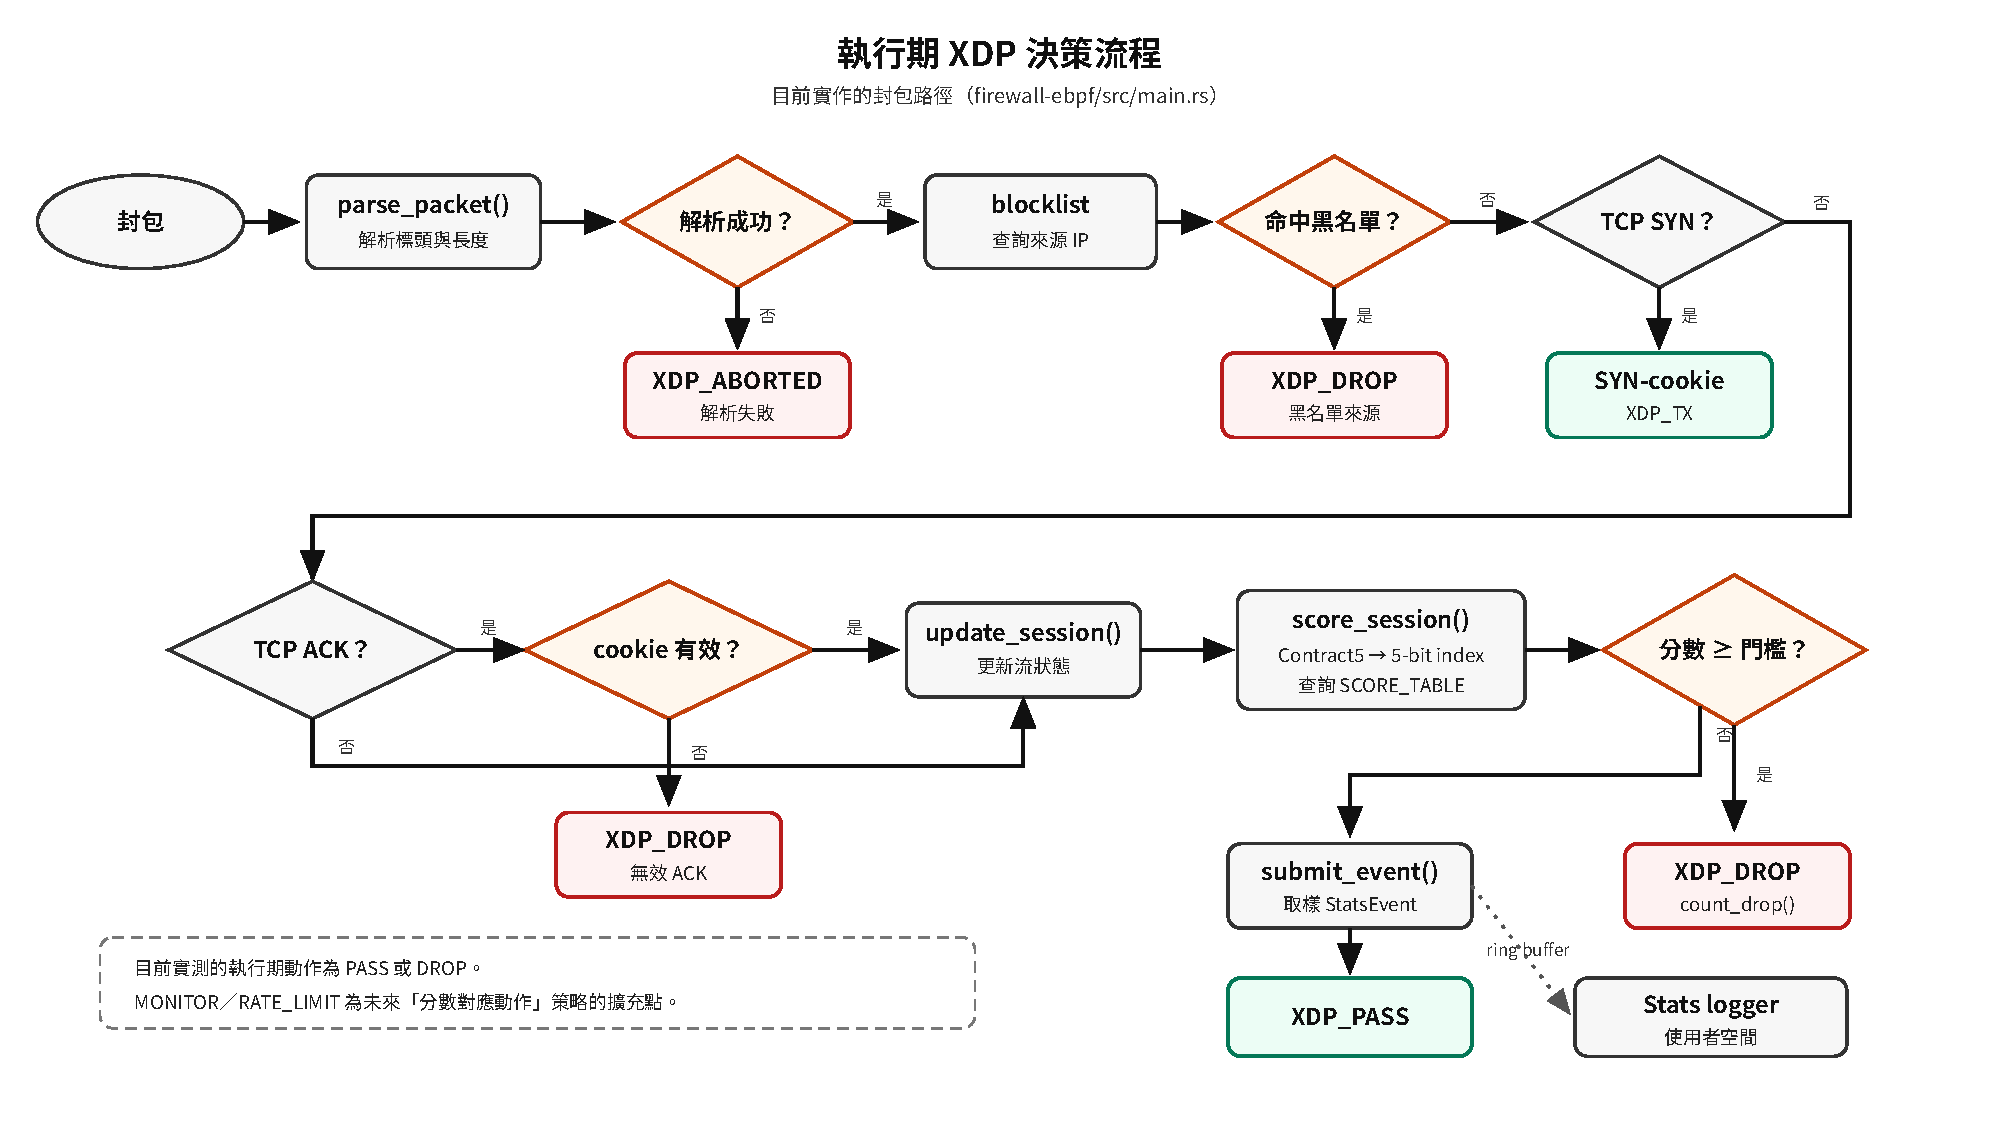
\includegraphics[width=0.95\textwidth]{figures/runtime_datapath.pdf}
  \caption{目前 XDP 執行期封包決策流程。封包經解析、黑名單、SYN-cookie 與連線狀態更新後，由 \code{score\_session()} 產生 5-bit index 並查詢 score table；現況 runtime action 為 \code{PASS} 或 \code{DROP}。}
  \label{fig:runtime-datapath}
\end{figure}

\subsection{模型部署規格與 BPF map 載入}
部署模型以 JSON 形式載入使用者空間，並由 Rust 載入器驗證中介資料後寫入 BPF map。模型格式包含 \code{version}、\code{feature\_order}、\code{threshold\_cmp}、\code{score\_scale}、\code{length\_unit}、\code{threshold}、\code{quantile\_bounds} 與 \code{score\_table}。其中特徵順序必須固定為 \code{protocol}、\code{pkt\_len\_mean}、\code{fwd\_max\_q}、\code{sym\_ratio}、\code{pkt\_cv\_sq}，且位元順序採最低有效位元優先（least-significant bit first）：

\begin{equation}
\begin{aligned}
idx ={}& (protocol\_bit \ll 0) \\
     |{}& (pkt\_len\_mean\_bit \ll 1) \\
     |{}& (fwd\_max\_q\_bit \ll 2) \\
     |{}& (sym\_ratio\_bit \ll 3) \\
     |{}& (pkt\_cv\_sq\_bit \ll 4).
\end{aligned}
\end{equation}

此規格禁止隱含的特徵順序，並要求 \code{score\_table} 長度為 32、\code{quantile\_bounds} 長度為 5。若 JSON 中介資料不符合規格，使用者空間載入器應拒絕載入，以避免 Python 離線流程、Rust 控制面與 eBPF 評分器之間產生無聲的規格不一致（silent mismatch）。

\subsection{離線機器學習流程}
離線機器學習流程使用 CIC-IDS-2019 僅正常（BENIGN-only）訓練資料建立孤立森林相關模型，並產出核心可用的分位桶邊界與評分表。本研究區分三種 model class：Contract5 continuous teacher 作為 teacher / reference model；Abs20／Full25 作為不可部署的 baseline upper bound；deployed binarized student 則是 5-bit 全二值化 32-entry 查表模型。現況部署表由二值特徵模型產生；第~\ref{sec:kd-granularity} 節進一步以 per-bucket teacher-score aggregation 實作正式 Contract5 continuous teacher 到 bucket student 之 knowledge distillation 對照，結果顯示在 $N=2$ 部署粒度下其偵測操作點與現況二值化流程幾乎等價。因此，本報告使用 quantile-bucket distillation 描述將離線異常偵測邏輯壓縮為核心查表部署格式的工程流程，並以正式 KD 對照確認目前部署捷徑並未損失低 FPR 操作點下的偵測能力。

\begin{figure}[H]
  \centering
  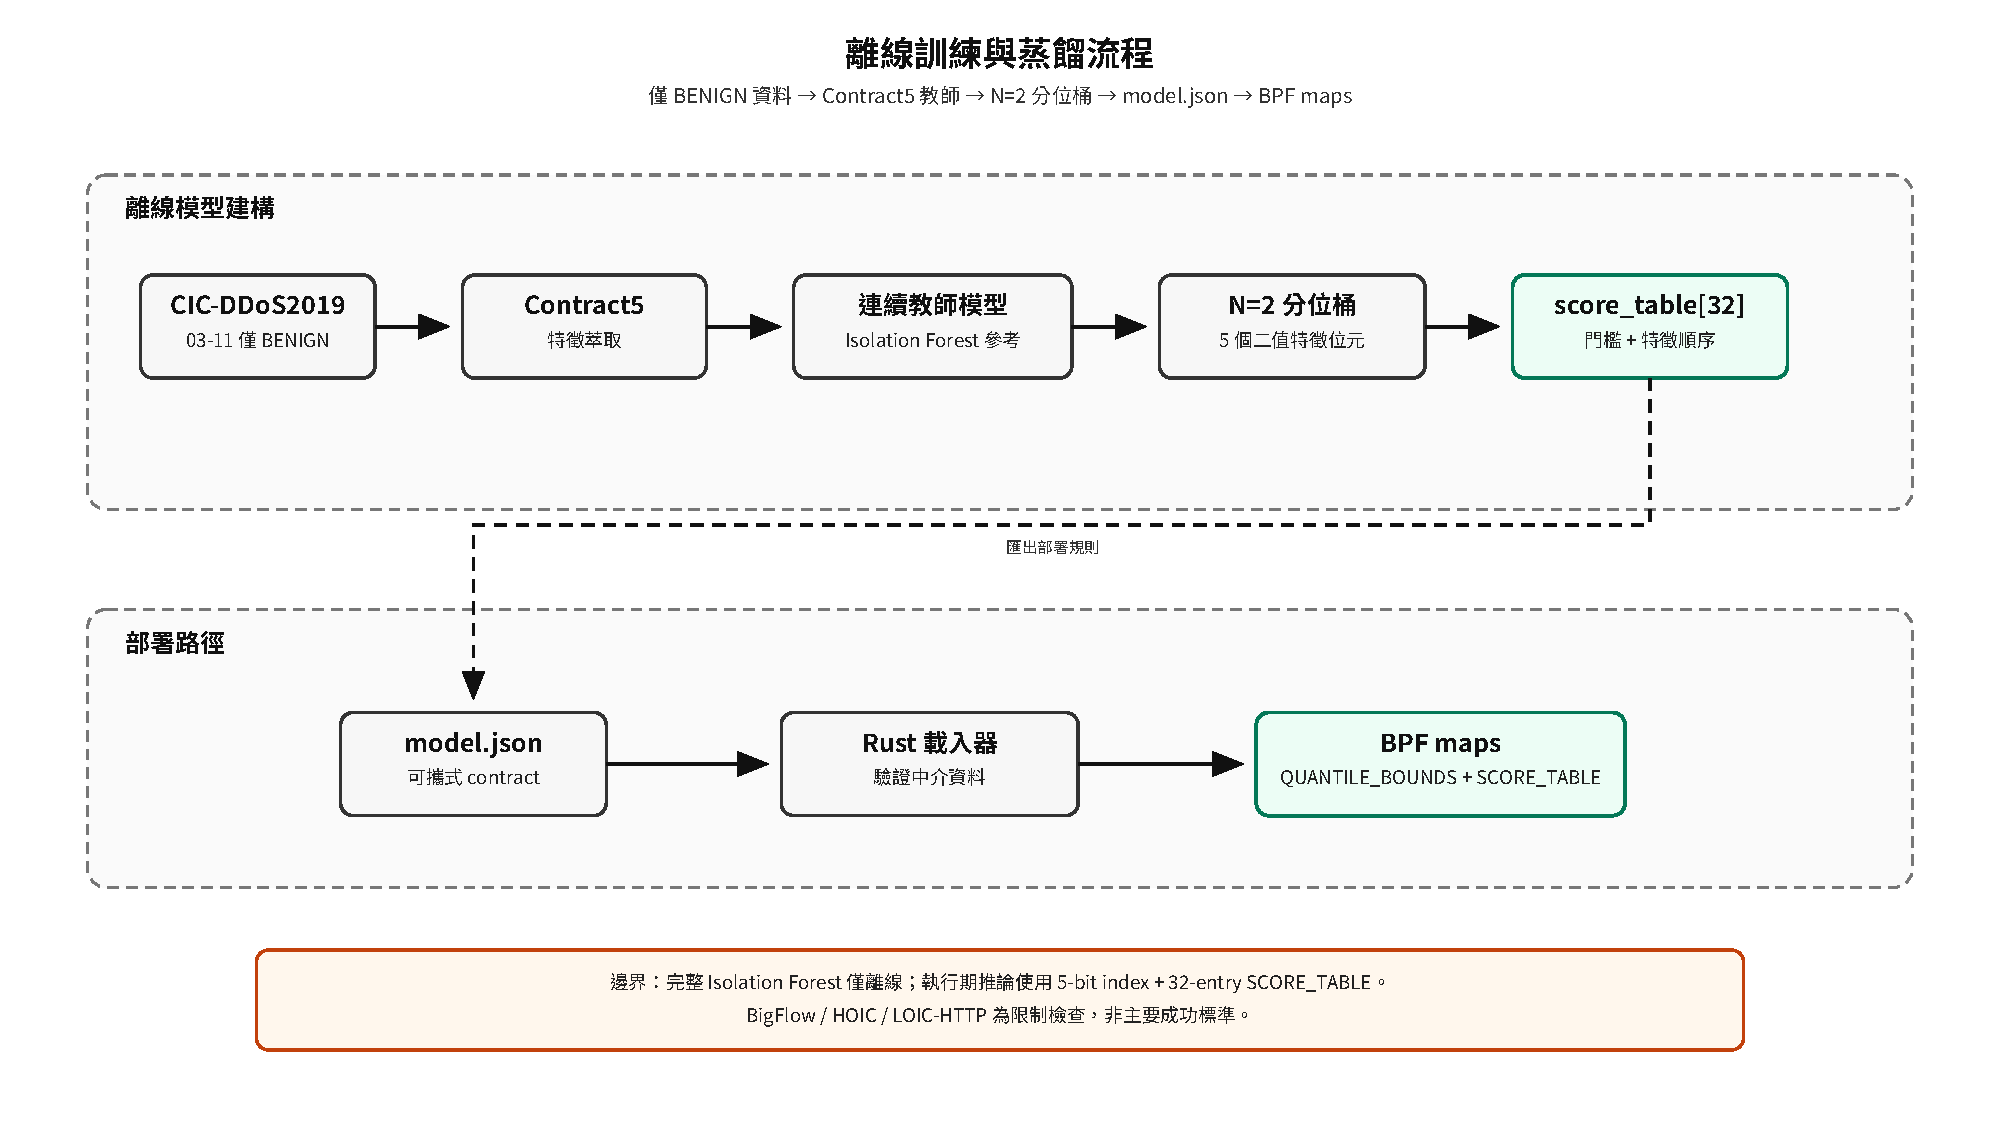
\includegraphics[width=0.95\textwidth]{figures/offline_pipeline.pdf}
  \caption{離線訓練與部署表產生流程。BENIGN-only 資料先轉換為 Contract5 特徵並訓練 continuous teacher，再以 $N=2$ 分位桶形成 5-bit index、32-entry score table 與 \code{model.json}，最後由 Rust loader 載入 BPF maps。}
  \label{fig:offline-pipeline}
\end{figure}

\subsection{資料集與評估 Protocol}
\label{sec:eval-protocol}
本研究的主成果採固定資料切分與操作點評估，避免以測試集最佳化門檻誇大效果。訓練資料使用 CIC-IDS-2019 中 03-11 檔案的 BENIGN 流量，並以 BENIGN-only 原則訓練無監督 Isolation Forest 與分位桶邊界；評估資料使用 01-12 檔案，抽取 BENIGN 與各攻擊類型樣本形成平衡式評估集。表~\ref{tab:eval-protocol} 摘要本報告所有主要偵測實驗共用的 protocol。

\begin{table}[H]
  \centering
  \caption{資料集與評估 protocol 摘要}
  \label{tab:eval-protocol}
  \small
  \renewcommand{\arraystretch}{1.2}
  \begin{tabularx}{\textwidth}{l X}
    \toprule
    \textbf{項目} & \textbf{設定} \\
    \midrule
    主資料範圍 & CIC-IDS-2019 / CIC-DDoS2019；BigFlow、IDS2018 HOIC 與 LOIC-HTTP 僅作分佈轉移與限制分析，不作主要成功標準 \\
    訓練資料 & 03-11 BENIGN-only flow；避免 IF 訓練資料混入 attack label \\
    評估資料 & 01-12 BENIGN + DDoS attack flows；主要 benchmark 評估列數約 48k，逐攻擊表中每類約 4000 筆，WebDDoS 因資料量限制為 439 筆 \\
    操作點 & 以 FPR $\leq 1\%$ 作為主要門檻選擇與回報標準，重點觀察 Precision、Recall、F1、FPR 與 FNR，而非僅比較 ROC-AUC \\
    部署回放 & legitimate drop ratio 另以實際 ship 的 \code{model.json} 固定 threshold = 7073 進行離線回放；此數字不同於重校準至 FPR $\leq 1\%$ 的理想操作點 \\
    Runtime 對齊 & kernel fast path 使用同一 5-bit index、32-entry \code{score\_table} 與 \code{score >= threshold -> DROP} 判定條件；完整 IF 僅作離線 teacher / reference model \\
    \bottomrule
  \end{tabularx}
\end{table}

\subsection{邊界更新器與事件回饋}
使用者空間回饋層透過核心送出的 \code{StatsEvent} 取得流層級分數、特徵分子／分母與良性閘門旗標。Rust 的 \code{BoundaryUpdater} 同時維護 \code{S\_ref} 與 \code{S\_live} 兩個草圖：\code{S\_ref} 僅接收低風險樣本，用以代表可信的參考分布；\code{S\_live} 則接收目前取樣視窗中的整體樣本，用以觀察當前流量分布。當散度或高風險分位桶跳變顯示疑似攻擊污染時，閘門狀態會進入 AttackFreeze，凍結參考邊界；若判定為正常漂移，則以指數移動平均（EMA）緩慢更新邊界。

邊界寫回採具版本號的雙緩衝 BPF map：使用者空間先寫入未啟用緩衝區，再更新中介資料切換啟用緩衝區，避免核心讀到半更新狀態。此機制更新的是分位桶邊界與分數對策略的映射，而不是在線上重新訓練孤立森林。

\subsection{實作狀態與驗證邊界}
目前核心資料結構、XDP／TC 資料路徑、模型 JSON 載入、評分表查表、邊界更新器狀態機與可於主機測試的整合流程已實作。Linux 端曾完成基本端到端執行，包含 eBPF 程式載入、XDP／TC 掛載、日誌環形緩衝區（ring buffer）讀取與優雅關閉（graceful shutdown）。吞吐量、每秒封包數（pps）、CPU 額外負擔、XDP 單次調用成本與 map update latency 已於 loopback 測試平台完成初步量測（見第~\ref{sec:results} 章）。legitimate drop ratio 亦已以部署評分路徑的離線回放補齊（CIC-DDoS2019 benign + attack 混流、固定 threshold，0.57\%）。仍待補充的是自適應邊界觸發與黑名單行為的實機驗證，以及實體網卡 native XDP 的線速基準。因此，本報告在成果章節僅將目前系統定位為可部署的快速路徑雛形與範圍內實驗驗證，而不宣稱完整的生產級 DDoS 防護基準測試已完成。

% =============================================================
\section{成果與討論}
\label{sec:results}

\subsection{研究問題與證據對應}
成果章依導論提出的四項研究問題組織實驗證據。表~\ref{tab:rq-evidence} 先列出每個研究問題對應的主要表格與回答方式，避免將偵測、部署、效能與回饋層實驗混為單一準確率比較。

\begin{table}[H]
  \centering
  \caption{研究問題與實驗證據對應}
  \label{tab:rq-evidence}
  \small
  \renewcommand{\arraystretch}{1.2}
  \begin{tabularx}{\textwidth}{p{0.23\textwidth} p{0.32\textwidth} X}
    \toprule
    \textbf{研究問題} & \textbf{主要證據} & \textbf{回答方式} \\
    \midrule
    離線異常偵測邏輯與 eBPF 相容性 & 表~\ref{tab:main-results}、\ref{tab:formal-kd}、\ref{tab:kd-granularity}、\ref{tab:k-sweep} & 以 Contract5 與 $N=2$ 分位桶將完整 IF 壓縮為 32-entry 查表模型，並證明其在 FPR $\leq 1\%$ 操作點下可用 \\
    特徵整數化與比例比較 & 表~\ref{tab:features}、模型部署規格與 5-bit index 公式 & 以固定特徵順序、整數比較與交叉乘法表示比例特徵，避免核心快速路徑中的浮點與高成本除法 \\
    資料路徑分工與效能隔離 & 圖~\ref{fig:arch}、表~\ref{tab:hardware-perf-plan} & 目前實作將 scoring 放在 XDP fast path，TC 保留為 classifier 擴充點；loopback 量測顯示完整 bucket 路徑未造成吞吐崩潰 \\
    適應性邊界校準與攻擊污染隔離 & 表~\ref{tab:drift-gated}、\ref{tab:contamination} & 雙草圖閘控更新在攻擊污染下觸發 AttackFreeze，避免 naive streaming update 將攻擊流量校準為正常 \\
    \bottomrule
  \end{tabularx}
\end{table}

\subsection{硬軟體規格}
表~\ref{tab:spec} 為本專題實際驗證環境。由於 eBPF 驗證器行為與核心版本、clang／LLVM 版本及網卡驅動有關，所有實機量測均以此環境為準；離線訓練套件版本則以 \code{uv --project service/model} 所管理的 Python 環境為準。需特別說明的是，本機網路介面為無線網卡（Intel Wi-Fi 6E AX210，iwlwifi 驅動），該驅動不支援 driver-native XDP，XDP 程式僅能以 generic mode（skb 路徑）掛載於實體介面；因此實機效能量測規劃採 loopback／veth 拓樸進行（veth 驅動支援 native XDP），以避免無線實體層速率與 generic mode 的額外封包複製成本干擾資料路徑成本的量測。
\begin{table}[H]
  \centering
  \caption{實驗硬軟體環境規格}
  \label{tab:spec}
  \renewcommand{\arraystretch}{1.3}
  \begin{tabularx}{\textwidth}{l X}
    \toprule
    \textbf{項目} & \textbf{規格} \\
    \midrule
    CPU              & Intel Core i5-14400F（10 核 16 執行緒） \\
    記憶體           & 32\,GiB \\
    網路卡           & Intel Wi-Fi 6E AX210 無線網卡（iwlwifi 驅動；無 native XDP，generic mode 掛載） \\
    作業系統 / 核心版本 & Manjaro Linux / Linux 6.12.91（eBPF 需 Linux 5.x 以上） \\
    eBPF 工具鏈      & clang 22.1.5、libbpf 1.7.0、bpftool v7.7.0 \\
    使用者空間語言   & Rust（rustc 1.93.0） \\
    離線訓練環境     & Python 3.12.12，scikit-learn 1.8.0、Polars 1.38.1、Pandas 3.0.1 \\
    \bottomrule
  \end{tabularx}
\end{table}

\subsection{實驗目標與變數}
本研究的主成果以 CIC-IDS-2019 範圍內評估為準，並將操作點固定於 FPR $\leq 1\%$，避免使用最佳化於測試集的門檻造成過度樂觀。實驗比較 Contract5 continuous teacher、Abs20 baseline、deployed binarized 32-entry student，以及監督式 Logistic Regression／Random Forest 參考上界。此處的成功標準不是跨資料集平均 AUC，而是部署模型是否能在低 FPR 操作點維持高偵測能力，並同時滿足 eBPF fast path 的可部署性。其中監督式模型僅作為同特徵空間下的參考上界，用以判斷 Contract5 特徵本身的可分性，而非本系統的部署路徑。

\begin{table}[H]
  \centering
  \caption{CIC-DDoS2019 範圍內偵測能力（操作點 FPR $\leq 1\%$）}
  \label{tab:main-results}
  \small
  \renewcommand{\arraystretch}{1.15}
  \setlength{\tabcolsep}{3.5pt}
  \begin{tabular}{l l c c c c c c c}
    \toprule
    \textbf{模型} & \textbf{角色} & AUC & PR-AUC & P & R & F1 & FPR & FNR \\
    \midrule
    Contract5 IF & teacher & 0.845 & 0.984 & 0.987 & 0.059 & 0.112 & 0.009 & 0.941 \\
    Abs20 IF & baseline & 0.892 & 0.983 & 0.991 & 0.102 & 0.186 & 0.010 & 0.898 \\
    32-entry student & deployed & 0.897 & 0.990 & 0.999 & 0.821 & 0.901 & 0.007 & 0.179 \\
    Logistic Regression & 監督式參考 & 0.948 & 0.995 & 0.999 & 0.806 & 0.892 & 0.010 & 0.194 \\
    Random Forest & 監督式參考 & 0.934 & 0.993 & 1.000 & 0.817 & 0.900 & 0.000 & 0.183 \\
    \bottomrule
  \end{tabular}
\end{table}

由表~\ref{tab:main-results} 可知，deployed 5-bit 32-entry student 在 FPR $<1\%$ 的操作點達到 F1 = 0.901、Recall = 0.821 與 FPR = 0.007，與監督式 Random Forest／Logistic Regression 的操作點表現相近。此結果顯示，分位桶二值化在本範圍內環境中並非單純造成資訊損失；相反地，它將攻擊流量推入特定高分分位桶，使其在嚴格 FPR 操作點下比 continuous teacher 更容易形成可用門檻。換言之，本系統的價值不在忠實複製 teacher 的連續分數排序，而在於產生可於 kernel fast path 執行且操作點穩健的查表式決策。需說明的是，表~\ref{tab:main-results} 與後續表~\ref{tab:k-sweep} 中 $N=2$ 一列的數值（F1 = 0.900、Recall = 0.819）存在約 0.001--0.002 的差異，係因兩組實驗採不同隨機種子與取樣切分所致，不影響結論。

\subsection{Score Regression 與 Bucket Student 對照}
為確認 deployed student 的價值不是單純來自「更忠實地複製 teacher score」，本研究另比較直接回歸 Contract5 continuous teacher score 的 score-regression student 與部署用 bucket student。此實驗不以 ground-truth label 訓練 student，而是觀察 student output 與 teacher score ranking 的一致性，以及在 FPR $\leq 1\%$ 操作點下的偵測表現。

\begin{table}[H]
  \centering
  \caption{Score regression vs. bucket student（CIC-DDoS2019，FPR $\leq 1\%$）}
  \label{tab:regression-vs-bucket}
  \renewcommand{\arraystretch}{1.2}
  \begin{tabular}{l c c c c}
    \toprule
    \textbf{模型} & ROC-AUC & F1@1\% & Recall@1\% & Spearman $\rightarrow$ teacher \\
    \midrule
    teacher（Contract5 continuous） & 0.845 & 0.112 & 0.059 & 1.000 \\
    student-regression（MSE $\rightarrow$ teacher） & 0.857 & 0.111 & 0.059 & 0.990 \\
    student-bucket（32-entry） & 0.896 & 0.902 & 0.821 & 0.549 \\
    \bottomrule
  \end{tabular}
\end{table}

表~\ref{tab:regression-vs-bucket} 顯示，直接回歸 teacher score 雖能高度保留 teacher ranking（Spearman = 0.990），但也繼承了 teacher 在低 FPR 操作點下 Recall 偏低的問題。相對地，bucket student 並未忠實複製 teacher 的連續分數排序，卻能在操作點上取得 F1 = 0.902 與 Recall = 0.821。此結果修正了「分位桶保留 teacher ranking」的直覺假設：本系統的部署價值更接近於透過中位數二值化重塑分數分布，使攻擊流量集中於少數高分桶，進而產生核心端可查表且操作點可用的決策規格。

\subsection{正式 KD 對照與桶粒度敏感度}
\label{sec:kd-granularity}
為進一步檢驗現況部署表由二值特徵模型產生是否只是工程捷徑，本研究加入正式 teacher-student KD 對照。由於 bucket student 的輸入空間已被五個二值特徵完整切成 32 個 bucket，在任何每桶單一輸出的 student 中，對 teacher score 的均方或分布匹配目標都會退化為 per-bucket teacher-score aggregation：每個 bucket 的最佳輸出即為該 bucket 內 teacher 分數的聚合值。因此，本實驗固定與部署模型相同的 bucket boundary 與評估切分，僅將 score table 改由 Contract5 continuous teacher score 聚合產生，並與現況 binarized 32-entry table 對照。

\begin{table}[H]
  \centering
  \caption{正式 KD 與部署 32-entry student 對照（CIC-DDoS2019，FPR $\leq 1\%$）}
  \label{tab:formal-kd}
  \small
  \renewcommand{\arraystretch}{1.2}
  \begin{tabular}{l c c c c}
    \toprule
    \textbf{模型} & ROC-AUC & F1@1\% & Recall@1\% & Spearman $\rightarrow$ teacher \\
    \midrule
    teacher（Contract5 continuous） & 0.845 & 0.112 & 0.059 & 1.000 \\
    student-KD（per-bucket aggregation） & 0.870 & 0.901 & 0.821 & 0.556 \\
    student-binarized（部署 32-entry） & 0.896 & 0.902 & 0.821 & 0.549 \\
    \bottomrule
  \end{tabular}
\end{table}

表~\ref{tab:formal-kd} 顯示，正式 KD 並未使 student 更接近 teacher 的低 FPR 操作點；相反地，其 F1 與 Recall 幾乎與部署 binarized student 相同。這代表在 $N=2$ 的 32-entry contract 下，偵測能力主要來自 bucket partition 對分數分布的重塑，而非 score table 是由二值化 IF 或 teacher 聚合所產生。KD 的 Spearman $\rightarrow$ teacher 仍只有 0.556，亦說明它並未忠實保留 teacher ranking；因此，正式 KD 對目前部署操作點而言近似 no-op，而不是尚未補齊的關鍵缺口。

接著，本研究檢驗「KD 與 binarized 近似等價是否只是因為 32 桶太粗」的假設。若低 Spearman 主要由桶數太少造成，則將每個特徵的分位桶數從 $N=2$ 提高到 $N=4$ 或 $N=8$ 時，KD 的 Spearman $\rightarrow$ teacher 應顯著上升。表~\ref{tab:kd-granularity} 顯示結果並非如此。

\begin{table}[H]
  \centering
  \caption{KD 保真度與桶粒度敏感度（CIC-DDoS2019，FPR $\leq 1\%$）}
  \label{tab:kd-granularity}
  \small
  \renewcommand{\arraystretch}{1.2}
  \begin{tabular}{c r c c c c c}
    \toprule
    $N$ & \textbf{表大小} & fallback & KD F1@1\% & bin F1@1\% & KD Spearman & bin Spearman \\
    \midrule
    2 & 32 & 0.0\% & 0.900 & 0.901 & 0.556 & 0.549 \\
    4 & 1024 & 0.0\% & 0.901 & 0.000 & 0.558 & 0.534 \\
    8 & 32768 & 0.1\% & 0.000 & 0.899 & 0.555 & 0.546 \\
    \bottomrule
  \end{tabular}
\end{table}

表~\ref{tab:kd-granularity} 反駁「桶太少導致 KD 不保真」的解釋：KD Spearman 從 32 桶到 32768 桶皆維持在約 0.555，並未隨粒度提高而接近 teacher。這表示 Contract5 feature contract 本身已限制可保留的 teacher ranking；增加桶數無法恢復 teacher 分數中未被這五個可部署特徵表達的排序資訊。另一方面，細粒度 bucket 會引入新的低 FPR 操作點脆弱性：$N=4$ 時 binarized 填表在 FPR $\leq 1\%$ 下崩潰，$N=8$ 時則改由 KD 填表崩潰。故 $N=2$ 不只是 eBPF table size 的折衷，也是目前在兩種填表方法下皆能維持穩定操作點的甜蜜點。

\subsection{逐攻擊類型分析}
\begin{table}[H]
  \centering
  \caption{Deployed student recall by CIC-DDoS2019 attack type（FPR $\leq 1\%$）}
  \label{tab:per-attack}
  \renewcommand{\arraystretch}{1.2}
  \begin{tabular}{l c c}
    \toprule
    \textbf{Attack type} & \textbf{Samples} & \textbf{Deployed student Recall} \\
    \midrule
    DrDoS\_DNS & 4000 & 1.000 \\
    DrDoS\_LDAP & 4000 & 1.000 \\
    DrDoS\_MSSQL & 4000 & 1.000 \\
    DrDoS\_NTP & 4000 & 0.998 \\
    DrDoS\_NetBIOS & 4000 & 0.999 \\
    DrDoS\_SNMP & 4000 & 1.000 \\
    DrDoS\_SSDP & 4000 & 1.000 \\
    DrDoS\_UDP & 4000 & 1.000 \\
    TFTP & 4000 & 0.993 \\
    Syn & 4000 & 0.000 \\
    UDP-lag & 4000 & 0.131 \\
    WebDDoS & 439 & 0.000 \\
    \bottomrule
  \end{tabular}
\end{table}

表~\ref{tab:per-attack} 顯示部署快速路徑對 UDP 反射／放大類型攻擊與 TFTP 達 99\% 以上 Recall，符合本系統鎖定高流量型 DDoS 的威脅模型。相對地，Syn、UDP-lag 與 WebDDoS 為明確盲區：Syn 類攻擊另由 SYN-cookie 路徑處理，不以分位桶評分器作為主要偵測手段；UDP-lag 與 WebDDoS 則需要不同特徵或更高層語意，並非目前 Contract5 快速路徑的主目標。此外，同一 Contract5 特徵空間下的監督式參考模型亦呈現相同盲區，顯示這些失效主要來自目前特徵契約的表達能力限制，而非單純由無監督訓練造成。

\subsection{離線推論成本對照}
本節僅比較模型壓縮前後在使用者空間 proxy 中的 per-flow 推論成本，用以說明完整 IF 與查表式推論的成本量級差異，而非宣稱核心端實機延遲。表~\ref{tab:inference-cost} 的查表數字包含 Python／資料處理開銷，因此可視為相對保守的查表成本上界；實際核心端仍需待後續實機量測補齊 pps、CPU 額外負擔與 map lookup latency。

\begin{table}[H]
  \centering
  \caption{模型推論成本對照（per-flow，userspace proxy）}
  \label{tab:inference-cost}
  \renewcommand{\arraystretch}{1.2}
  \begin{tabularx}{\textwidth}{l c X}
    \toprule
    \textbf{路徑} & \textbf{延遲（$\mu$s / flow）} & \textbf{說明} \\
    \midrule
    Contract5 IF per-flow 推論 & 5948.2 & 使用者空間完整 Isolation Forest 推論，代表未壓縮模型的參考成本 \\
    Contract 整數查表 & 33.6 & 使用者空間 proxy 查表，包含 Python／資料處理開銷，作為保守上界 \\
    加速比（IF / 查表） & 177$\times$ & 支撐「查表推論成本遠低於完整 IF」的方向性結論 \\
    \bottomrule
  \end{tabularx}
\end{table}

此結果不等同於已完成核心端奈秒級延遲或整機吞吐量基準測試；其意義在於確認模型壓縮後的整數查表路徑相較完整 IF 推論具有明顯成本差距。核心端的實機吞吐量、CPU 使用率、XDP 路徑延遲與偵測迴圈延遲，於下一小節以 loopback 測試平台量測。

\subsection{實機效能量測（loopback 測試平台）}
本節於表~\ref{tab:spec} 主機上以 loopback 拓樸（XDP 以 xdpgeneric 掛載於 \code{lo}）實際量測核心端 fast-path 成本，流量由 \code{hping3 --flood} 單核產生，腳本為 \code{scripts/bench/}（throughput、map\_latency、mitigation\_latency）。結果如表~\ref{tab:hardware-perf-plan}，每項取多次重跑的代表值。

最具意義的核心端數字是 XDP 程式的單次調用成本：以 \code{kernel.bpf\_stats\_enabled} 取 \code{run\_time\_ns}／\code{run\_cnt} 比值，得到每個封包通過整支 XDP 程式（封包解析、黑名單查表、連線狀態更新與 32-entry 評分表查表）約 410\,ns（跨兩日七次重跑 394--428\,ns，最終穩定輪 416.5\,ns）。對照表~\ref{tab:inference-cost} 的 userspace 完整 IF 推論（每流 5948.2\,$\mu$s，單核換算上限約 168 flows/s），核心端整數查表路徑與 userspace 樹狀推論之間存在約四個數量級的處理速率差距，與本系統「將推論壓入核心快速路徑」的訴求一致。

惟須誠實界定三項量測限制，以免高估結論：（一）單機 loopback 的封包產生受限於單核 \code{hping3}，實測上限約 1.0--1.13\,Mpps（\code{setup\_testbed} 探測值 1.02\,Mpps，隨背景負載浮動），因此各對照組的吞吐皆觸及\textbf{產生器天花板而非防火牆天花板}；可得的結論是「啟用完整 eBPF bucket 資料路徑不會造成吞吐崩潰」（最終穩定輪 1.04\,Mpps vs.\ no-mitigation 1.13\,Mpps，差距約 8\%；前一輪 1.00 vs.\ 1.02\,Mpps，差距 $<2\%$），而非防火牆的最大可承受封包率。（二）CPU\% 為單機數值，流量產生器與防火牆共用核心，故各組 CPU\% \textbf{不可直接相互比較}為 enforcement 淨額外負擔。（三）表中 mitigation latency 約 200\,ms 是「使用者空間以 \code{bpftool} 輪詢偵測首個 DROP」的迴圈延遲，由 \code{hping3} 程序啟動與 map dump 輪詢主導，\textbf{並非核心端封包丟棄延遲}；核心端對命中黑名單封包的丟棄即發生於上述單次 XDP 調用（約 410\,ns）內。Map update latency 則以直接微基準量測：對已載入核心的 QUANTILE\_BOUNDS／BOUNDARY\_META 連續呼叫 \code{write\_boundary\_version}（雙緩衝寫入＋版本切換），p50 約 2--3\,$\mu$s、p99 約 3\,$\mu$s（表~\ref{tab:hardware-perf-plan}）；之所以用微基準而非自然觸發，是因為自適應閘控\textbf{僅在 benign 主導的流量下才發布}邊界更新（純攻擊流量會使 reference 批次無法湊滿而凍結，即 AttackFreeze 設計），於 loopback 合成流量難以自然觸發該路徑。最後，legitimate drop ratio（in-the-wild 誤丟率）以離線回放補齊：用實際 ship 的 \code{model.json} 固定 threshold（與 kernel \code{score}$\geq$threshold $\to$ DROP 完全相同的判定條件），在 CIC-DDoS2019 benign + attack 混流（每類 4000 筆）上比對 ground-truth label，得正常流誤丟 23/4000＝\textbf{0.57\%}。需強調此為部署評分路徑的離線回放（非線上封包量測），但其判定邏輯與核心端一致；該數字亦與表~\ref{tab:main-results} 的 FPR = 0.007 互為印證——後者是重校準至 FPR $\leq 1\%$ 操作點的理想值，本數字則為固定 threshold = 7073 下的實際誤丟率。整條串流視角下，legitimate drop ratio 與攻擊混入比例無關（per-flow 獨立評分），但「被丟流量中誤丟正常流的占比」（false-drop share）會隨攻擊稀少而上升：攻擊佔 10\% 時約 5.9\%、佔 80\% 時降至 0.18\%。

\begin{table}[H]
  \centering
  \caption{實機效能量測結果（loopback 測試平台，CIC-DDoS2019 威脅模型）}
  \label{tab:hardware-perf-plan}
  \small
  \renewcommand{\arraystretch}{1.3}
  \setlength{\tabcolsep}{4pt}
  \begin{tabularx}{\textwidth}{%
      >{\raggedright\arraybackslash}p{0.16\textwidth}%
      >{\raggedright\arraybackslash\hsize=0.85\hsize}X%
      >{\raggedright\arraybackslash\hsize=1.15\hsize}X}
    \toprule
    \textbf{量測項目} & \textbf{結果} & \textbf{說明} \\
    \midrule
    XDP 單次調用成本（ns） & $\approx$ 410（394--428，$n=7$） & 整支 XDP 程式每封包成本（解析＋黑名單＋連線更新＋評分表查表）；\code{bpf\_stats} run\_time\_ns/run\_cnt；最終穩定輪 416.5\,ns \\
    Packet throughput（pps） & eBPF bucket 1.04\,M；no-mitigation 1.13\,M；static-blocklist 0.75\,M（全丟棄路徑）；userspace IF $\approx$ 168\,flow/s & 最終穩定輪數值（前輪 eBPF bucket 0.88--1.02\,M、no-mitigation 0.93--1.02\,M 一致）；eBPF bucket 與 no-mitigation 觸及單核 hping3 產生上限，故為「不造成吞吐崩潰」之證據而非防火牆極限；userspace IF 由 $10^6/5948.2\,\mu$s 換算 \\
    CPU usage（\%） & no-mitigation 11.1；eBPF bucket 16.9；static-blocklist 9.5 & 最終穩定輪數值（多輪重跑 eBPF bucket 16--26、波動大）；單機數值，產生器與防火牆共用核心，不作組間淨負擔比較 \\
    Mitigation latency（偵測迴圈，ms） & 218（中位數，$n=10$；五輪中位數 196--223） & 由 hping3 啟動與 bpftool 輪詢主導，非核心丟棄延遲；核心端丟棄含於上列 410\,ns \\
    Map update latency（$\mu$s） & $\approx$ 2--3（p50；p99 $\approx$ 3） & \code{write\_boundary\_version} 一次發布成本（5 筆 QUANTILE\_BOUNDS \code{set} ＋ 1 筆 BOUNDARY\_META 版本切換）；3 輪 $\times$1000 次對 kernel map 直接微基準（p50 1.7/2.5/3.1、p99 2.6/2.9/3.2） \\
    Legitimate drop ratio（\%） & 0.57（離線回放） & 以部署 \code{model.json} 固定 threshold（kernel \code{score}$\geq$threshold $\to$ DROP 同條件）在 CIC-DDoS2019 benign + attack 混流上比對 ground-truth；正常流誤丟 23/4000。非線上封包量測，係部署評分路徑回放 \\
    \bottomrule
  \end{tabularx}
\end{table}

\subsection{分位桶數量選擇}
\begin{table}[H]
  \centering
  \caption{靜態分位桶數量敏感度（CIC-DDoS2019 範圍內）}
  \label{tab:k-sweep}
  \renewcommand{\arraystretch}{1.2}
  \begin{tabular}{c c c c c c}
    \toprule
    \textbf{N} & \textbf{eBPF 查表大小} & ROC-AUC & PR-AUC & F1@FPR$\leq$1\% & Recall@1\% \\
    \midrule
    2 & 32-entry & 0.894 & 0.989 & 0.900 & 0.819 \\
    4 & 1024-entry & 0.890 & 0.989 & 0.000 & 0.000 \\
    8 & 32768-entry & 0.908 & 0.991 & 0.899 & 0.817 \\
    \bottomrule
  \end{tabular}
\end{table}

$N=2$ 的選擇並非單純為了降低表大小而犧牲精度。表~\ref{tab:k-sweep} 顯示，$N=4$ 雖然 ROC-AUC 與 PR-AUC 看似正常，但在 FPR $\leq 1\%$ 的操作點完全崩潰；$N=8$ 雖可恢復操作點表現，但需要 32768-entry 表，對 eBPF 快速路徑的記憶體與驗證器負擔明顯不利。因此，$N=2$ 同時滿足 32-entry 小表、操作點穩健性與核心可行性，是目前部署規格的合理選擇。

\subsection{漂移情境下的邊界更新穩健性}
除了靜態偵測表現外，本研究也評估分位桶邊界在串流更新情境中的穩健性。此實驗比較三種策略：Static 使用訓練期邊界且不更新；Periodic 於每個視窗直接以當前流量重新計算邊界；Gated 則採用雙草圖與閘門狀態，只在判定為正常漂移時更新參考邊界，並於疑似攻擊污染時進入 AttackFreeze。

\begin{table}[H]
  \centering
  \caption{Static / Periodic / Gated under drift}
  \label{tab:drift-gated}
  \renewcommand{\arraystretch}{1.2}
  \begin{tabular}{c c c c c}
    \toprule
    \textbf{win} & \textbf{atk\%} & Static F1 / FNR & Periodic F1 / FNR & Gated F1 / FNR \\
    \midrule
    0 & 10\% & 0.876 / 0.185 & 0.868 / 0.192 & 0.876 / 0.185 \\
    1 & 20\% & 0.887 / 0.189 & 0.880 / 0.198 & 0.887 / 0.189 \\
    2 & 30\% & 0.896 / 0.176 & 0.000 / 1.000 & 0.896 / 0.176 \\
    3 & 40\% & 0.894 / 0.184 & 0.000 / 1.000 & 0.894 / 0.184 \\
    4 & 50\% & 0.898 / 0.179 & 0.000 / 1.000 & 0.898 / 0.179 \\
    \bottomrule
  \end{tabular}
\end{table}

表~\ref{tab:drift-gated} 顯示，未設閘門的 Periodic 更新在攻擊比例達 30\% 後即崩潰，F1 降至 0 且 FNR 升至 1.000，代表攻擊流量污染了重新估計的邊界。Static 與 Gated 則維持約 0.88--0.90 的 F1 與約 0.18 的 FNR。需誠實說明的是，在此漂移設定中 Static 本身並未明顯退化，原因是目前 Contract5 中的比例與無量綱特徵對良性 rate／size 漂移具有一定抵抗力；因此 Gated 的主要價值不是在本實驗中優於 Static，而是避免無閘門串流更新在攻擊污染下將攻擊校準為正常。

\subsection{資料漂移與攻擊污染防護}
本研究的自適應邊界並非線上重訓孤立森林，而是更新分位桶邊界與分數對策略的映射。此機制的核心風險是攻擊污染：若直接以目前視窗中的所有流量重新計算邊界，攻擊流量可能被納入新的參考分布，使攻擊被校準為正常。為此，系統採雙草圖閘控更新，僅讓通過良性閘門的低風險樣本進入 \code{S\_ref}，並以 \code{S\_live} 觀察當前整體分布。

\begin{table}[H]
  \centering
  \caption{攻擊污染掃描：樸素更新與閘控更新對照}
  \label{tab:contamination}
  \renewcommand{\arraystretch}{1.2}
  \begin{tabular}{c c c c c c}
    \toprule
    \textbf{攻擊比例 $\rho$} & 散度 & 高風險倍率 & 閘門決策 & 樸素 FNR & 閘控 FNR \\
    \midrule
    10\% & 0.349 & 34.6$\times$ & AttackFreeze & 0.190 & 0.182 \\
    30\% & 1.194 & 70$\times$ & AttackFreeze & 1.000 & 0.182 \\
    50\% & 2.224 & 89$\times$ & AttackFreeze & 1.000 & 0.182 \\
    80\% & 3.166 & 119$\times$ & AttackFreeze & 1.000 & 0.182 \\
    \bottomrule
  \end{tabular}
\end{table}

表~\ref{tab:contamination} 顯示，樸素串流更新在攻擊比例 $\rho \geq 30\%$ 時 FNR 上升至 1.000，代表攻擊流量已被更新後的邊界洗白為正常。相較之下，雙草圖閘控更新在所有測試比例下皆觸發 AttackFreeze，將 FNR 維持於基準值 0.182。此結果說明，在 DDoS 場景中，自適應機制若缺少污染隔離，反而可能破壞防禦邊界；閘控更新的核心價值在於保留邊界校準能力，同時避免攻擊流量污染參考邊界。

\subsection{成果定位與限制}
本專題的主要成果是建立一條可部署於 eBPF 資料路徑的低延遲機器學習式 DDoS 快速路徑：Contract5 特徵可由核心連線狀態重建，五個分位桶位元可組成 32-entry 評分表，並由 Rust 使用者空間進行模型載入與邊界更新。系統在 CIC-DDoS2019 上能有效覆蓋多數 UDP 反射／放大攻擊，但不宣稱解決所有 DDoS 型態。Syn、UDP-lag、WebDDoS 與跨資料集 HOIC／BigFlow 泛化皆屬限制或範圍外觀察。效能面已於 loopback 測試平台完成初步實機量測：XDP 每封包約 410\,ns、啟用完整 bucket 資料路徑不造成吞吐崩潰（1.04\,Mpps，達 baseline 約 92\%）；惟此為 xdpgeneric＋單核產生器環境，實體網卡 native XDP 與多核線速基準仍待最終驗證。

% =============================================================
\newpage
\section{結論與未來工作}
\label{sec:conclusion}

\subsection{結論}
本專題的核心結論是：DDoS 偵測模型若要進入 Linux kernel fast path，不能只追求離線準確率，而必須同時滿足 verifier-friendly、可由 datapath 重建、整數化、低推論成本與低誤報操作點等部署條件。基於此訴求，本專題提出並實作一條 Python 離線模型、Rust 使用者空間控制面與 eBPF XDP／TC 資料路徑三者對齊的低延遲 DDoS 偵測與初步處置管線。回應導論所提之四項研究問題：（一）在 eBPF 相容性方面，本系統以 Contract5 feature contract 與 $N=2$ 分位桶將五個特徵轉換為 5-bit 索引，並以 32-entry bucket student 評分表取代樹狀巡訪，使核心快速路徑僅需整數比較與查表；（二）在特徵整數化方面，比例特徵改以交叉乘法表示，避免浮點與高成本除法；（三）在資料路徑分工方面，目前實作由 XDP 負責封包解析、黑名單、SYN-cookie、狀態更新與分位桶評分，TC 保留為 classifier 擴充掛載點，避免完整模型進入 per-packet fast path；（四）在攻擊污染隔離方面，雙草圖閘控更新可在攻擊比例 $\rho \geq 30\%$ 時觸發 AttackFreeze，將 FNR 維持於基準值 0.182，而樸素更新則惡化至 1.000。

實驗以 CIC-IDS-2019 為範圍，deployed student 在 FPR $\leq 1\%$ 操作點達 F1 = 0.901、Recall = 0.821，與監督式 Random Forest／Logistic Regression 相近，並對多種 UDP 反射／放大型 DDoS 達 99\% 以上 Recall。進一步的對照實驗顯示，直接回歸 teacher score 雖能保留 teacher ranking，卻會繼承 teacher 在低 FPR 操作點下的不可用性；bucket student 反而透過離散化重塑分數分布，取得更可部署的操作點表現。正式 KD 對照亦顯示，per-bucket teacher-score aggregation 在 $N=2$ 下與現況 binarized 32-entry table 幾乎等價（F1 約 0.901、Recall 約 0.821），而提高桶粒度並未改善 KD 對 teacher ranking 的保真度，反而引入新的操作點脆弱性。分位桶數量敏感度因此顯示 $N=2$ 並非單純的 table size 妥協，而是操作點穩健性與 eBPF 可行性的交集；串流邊界實驗則說明，未設閘門的 Periodic 更新會在 attack contamination 下崩潰，而 Gated 更新可維持接近 Static 的乾淨基線。

整體而言，本專題的貢獻不在追求最高離線 AUC，而在於建立一條可驗證、可部署且操作點穩健的核心快速路徑偵測與初步處置管線，同時誠實界定其盲區與適用範圍。效能證據包含兩層：userspace 對照顯示查表式推論成本遠低於完整孤立森林推論（177$\times$）；loopback 實機量測則確認核心端 XDP 路徑每封包約 410\,ns、且完整 bucket 資料路徑不造成吞吐崩潰。legitimate drop ratio 以部署評分路徑離線回放測得固定 threshold 下正常流誤丟僅 0.57\%（與 Table~\ref{tab:main-results} 重校準操作點 FPR = 0.007 互為印證）；實體網卡 native XDP 線速基準仍需後續實機量測補齊。

\subsection{未來工作}
本研究尚有以下延伸方向：
\begin{itemize}
  \item \textbf{實體網卡與多核心效能驗證：} 目前 loopback 測試已確認 XDP fast path 每封包約 410\,ns 且完整 bucket 路徑不造成吞吐崩潰；後續需在實體網卡 native XDP、veth／雙機拓樸與多核心流量產生器下補齊線速基準，並區分整支 XDP invocation cost、單次 map lookup p50/p99 與真正 detection-to-drop latency。
  \item \textbf{KD 與特徵契約延伸：} 本研究已以 per-bucket teacher-score aggregation 驗證 $N=2$ 下正式 KD 與現況 binarized table 在低 FPR 操作點幾乎等價；後續若要進一步提升 teacher ranking 保真度，重點不應只放在增加桶數，而應評估新的 datapath 可重建特徵、灰區二階段模型或不同操作點校準策略。
  \item \textbf{Runtime Layer 2 推論：} 將完整 Isolation Forest 或其他較高成本模型接入 userspace，只針對 gray-zone、取樣上報或未來 \code{MONITOR} policy 標記的 flow 進行二階段判斷，避免讓完整模型進入 per-packet fast path。
  \item \textbf{盲區與多層防線擴充：} 針對 UDP-lag、WebDDoS／LOIC-HTTP 等目前 Contract5 無法表達的攻擊型態，研究可由 datapath 重建的新特徵或 userspace／application-layer 語意；對 SYN flood 則進一步驗證 SYN-cookie path 與 XDP bucket scorer 之間的分工。
  \item \textbf{控制面熱更新與 AttackFreeze 實機驗證：} 於實機流量重放環境驗證 gated update、AttackFreeze 觸發與 versioned double-buffer map update，並比較 direct update 與 versioned update 在高速封包通過時的 inconsistent decision count、stale policy duration 與封包處置一致性。
\end{itemize}

% =============================================================
\newpage
\begin{thebibliography}{99}

\bibitem{cloudflare2025q1ddos}
Cloudflare. ``Targeted by 20.5 million DDoS attacks, up 358\% year-over-year: Cloudflare's 2025 Q1 DDoS Threat Report.'' Cloudflare Blog, 2025. \url{https://blog.cloudflare.com/ddos-threat-report-for-2025-q1/}.

\bibitem{linuxBpfVerifier}
The Linux Kernel documentation. ``eBPF verifier.'' \url{https://docs.kernel.org/bpf/verifier.html}.

\bibitem{lai2022ebpf}
賴玠忠（2022）。\textit{基於 eBPF 之物聯網輕量監控機制的設計與實現}﹝碩士論文，國立政治大學﹞。臺灣博碩士論文知識加值系統。\url{https://hdl.handle.net/11296/9a28s3}。

\bibitem{sun2019ml}
孫維淋（2019）。\textit{植基於機器學習之分散式阻斷服務攻擊偵測}﹝碩士論文，國立高雄科技大學﹞。臺灣博碩士論文知識加值系統。\url{https://hdl.handle.net/11296/746r5s}。

\bibitem{zhao2024autoencoder}
趙奕勛（2024）。\textit{基於自編碼器重構誤差與孤立森林之未知分散式阻斷服務攻擊偵測}﹝碩士論文，國立高雄科技大學﹞。臺灣博碩士論文知識加值系統。\url{https://hdl.handle.net/11296/94azqr}。

\bibitem{wu2024dnn}
吳承恩（2024）。\textit{以深度神經網路和優化特徵提高 DDoS 攻擊檢測效果}﹝碩士論文，萬能科技大學﹞。臺灣博碩士論文知識加值系統。\url{https://hdl.handle.net/11296/spx9zx}。

\bibitem{remya2025ebpf}
S. Remya et al., ``eBPF-Based Runtime Detection of Semantic DDoS Attacks in Linux Containers,'' \textit{IEEE Access}, vol. 13, pp. 169178--169219, 2025, doi: 10.1109/ACCESS.2025.3614389.

\bibitem{verma2022feature}
J. Verma, A. Bhandari and G. Singh, ``Feature Selection Algorithm Characterization for NIDS using Machine and Deep learning,'' \textit{2022 IEEE International IOT, Electronics and Mechatronics Conference (IEMTRONICS)}, Toronto, ON, Canada, 2022, pp. 1--7, doi: 10.1109/IEMTRONICS55184.2022.9795709.

\bibitem{moyano2023feature}
R. F. Moyano et al., ``A Feature Selection Approach Towards the Standardization of Network Security Datasets,'' \textit{2023 IEEE 9th International Conference on Network Softwarization (NetSoft)}, Madrid, Spain, 2023, pp. 257--261, doi: 10.1109/NetSoft57336.2023.10175497.

\bibitem{li2024featureReduction}
J. Li, M. S. Othman, H. Chen, and L. M. Yusuf, ``Optimizing IoT intrusion detection system: feature selection versus feature extraction in machine learning,'' \textit{Journal of Big Data}, vol. 11, article 36, 2024, doi: 10.1186/s40537-024-00892-y. \url{https://doi.org/10.1186/s40537-024-00892-y}.

\bibitem{uddin2026bigflow}
Uddin, M. B., Arefin, M. S., \& Hussain, M. M. M. (2026). BigFlow-NIDS: A large-scale dataset for network intrusion detection in big data environment. \textit{Data in Brief}, 65, 112530. \url{https://doi.org/10.1016/j.dib.2026.112530}.

\bibitem{shahinfar2025demystifying}
Farbod Shahinfar, Sebastiano Miano, Aurojit Panda, and Gianni Antichi. 2025. Demystifying Performance of eBPF Network Applications. \textit{Proc. ACM Netw.} 3, CoNEXT3, Article 16 (September 2025), 21 pages. \url{https://doi.org/10.1145/3749216}.

\end{thebibliography}

\end{document}
